\documentclass[a4paper,10pt]{article}
\usepackage{enumitem}
\usepackage{titlesec}
\usepackage{geometry}
\usepackage{graphicx} 

\geometry{margin=1in}

\title{Spotify Documentation}
\date{}

\begin{document}
\section*{6- Stakeholders in a System or Application}

In the context of a system or application, stakeholders are individuals or groups that have an interest or stake in the project's outcome. Below is a breakdown of the two types of stakeholders, with examples relevant to a platform like Spotify:

\begin{itemize}
    \item \textbf{Primary Stakeholders:}
    
    These are the people who directly interact with and use the system. They are the main users whose needs and experiences are prioritized during the system's design and development.
    
    \begin{itemize}
        \item \textbf{Users:} The individuals who subscribe to and use Spotify to stream music, create playlists, and discover new content.
        
        \item \textbf{Admins:} The team members responsible for managing the platform’s operations, such as content moderation, user support, and system management.
    \end{itemize}

    \item \textbf{Secondary Stakeholders:}
    
    These are individuals or entities that have an interest in the system but do not directly use it as primary stakeholders do. They may influence or be affected by the system in various ways.
    
    \begin{itemize}
        \item \textbf{Partners:} Record labels, artists, and content creators who provide music and other content for Spotify.
        
        \item \textbf{Banks and Financial Institutions:} These entities handle financial transactions and payments for subscriptions, royalties, and other financial operations.
        
        \item \textbf{Advertisers:} Companies that purchase advertising space within the Spotify app to reach its user base.
    \end{itemize}
    
\end{itemize}

These stakeholders play different roles and have varying degrees of impact and influence on the system, contributing to its development, functionality, and success.


\maketitle

\section*{9 - User Requirements for a Spotify-Like Application}
This section outlines the essential user requirements for a Spotify-like application.

\subsection*{1. User Characteristics}
This section outlines the essential characteristics required for user accounts on the platform.

\begin{itemize}[leftmargin=*]
    \item \textbf{User ID and Username:} Each user must have a unique identifier and username to ensure distinct profiles and prevent duplication.
    \item \textbf{Age and Parental Controls:} The system will capture users’ ages and provide parental control options for younger users to monitor and manage accessible content.
    \item \textbf{Subscription and Payment Methods:} Users will have the option to select between free and premium subscriptions, with multiple flexible payment methods available.
    \item \textbf{Email and Contact Information:} Valid contact details, including email, are required for notifications and account recovery purposes.
    \item \textbf{Account Type:} Accounts will be categorized as either a regular User account or an Artist account, determining available features and functionalities.
\end{itemize}

\subsection*{2. Functional Requirements}
This section defines the key functionalities that the application must support.

\subsubsection*{2.1 User Management}
Functions related to managing user accounts and profiles.

\begin{itemize}[leftmargin=*]
    \item \textbf{Account Creation:} Users can register using email or phone, with an option for social media linked account sign-ins.
    \item \textbf{Profile Updates:} Users can update their profile information, including username, profile picture, and contact details.
    \item \textbf{Subscription Management:} Users can upgrade, downgrade, or cancel their subscriptions at any time, with corresponding feature adjustments.
    \item \textbf{Linked Accounts:} Users can link social media accounts to enhance connectivity and sharing options.
\end{itemize}

\subsubsection*{2.2 Music Streaming and Library Management}
Features related to music streaming and library organization.

\begin{itemize}[leftmargin=*]
    \item \textbf{Music Streaming:} The system shall provide free (with ads) and premium (ad-free) streaming options, with users controlling playback based on their subscription type.
    \item \textbf{Personalized Playlists:} Curated playlists tailored to user preferences and listening history will be offered (e.g., “Top Hits,” “Discover Weekly”).
    \item \textbf{Playlist Management:} Users can create, edit, and delete playlists, as well as add or remove songs.
    \item \textbf{Advanced Search:} Users can search for music by artist, title, genre, mood, and keywords for easy content location.
\end{itemize}

\subsubsection*{2.3 Social and Sharing Features}
Capabilities for users to interact and share their musical experiences.

\begin{itemize}[leftmargin=*]
    \item \textbf{Social Media Sharing:} Users can share playlists or songs on social media platforms through a visually appealing interface.
    \item \textbf{Follower and Following System:} Users can follow friends and artists to stay updated on new music and shared playlists.
    \item \textbf{Blending Feature:} Users can blend their music tastes with friends to explore common interests and discover new music.
    \item \textbf{Collaborative Playlists:} Users can co-create playlists with friends and listen together in real-time.
\end{itemize}

\subsection*{3. Non-Functional Requirements}
This section defines the performance criteria and constraints for the application.

\subsubsection*{3.1 Performance and Scalability}
Criteria for system performance and its ability to scale with user demand.

\begin{itemize}[leftmargin=*]
    \item \textbf{Load Time:} The system shall load songs within a maximum of 2 minutes to ensure a seamless user experience.
    \item \textbf{Search Query Performance:} The system shall efficiently handle a minimum of X concurrent search queries (replace X with a target number).
    \item \textbf{User Growth Management:} The system shall dynamically manage user growth to ensure consistent performance as the user base expands.
\end{itemize}

\subsubsection*{3.2 Usability and Accessibility}
Requirements ensuring the application is user-friendly and accessible to all.

\begin{itemize}[leftmargin=*]
    \item \textbf{User Interface Design:} The system shall feature an intuitive and user-friendly interface that facilitates easy navigation for all users.
    \item \textbf{Accessibility Standards:} The application shall comply with established accessibility standards, making it usable for individuals with disabilities and supporting multiple languages.
\end{itemize}

\subsubsection*{3.3 Security and Compliance}
Measures to protect user data and comply with legal requirements.

\begin{itemize}[leftmargin=*]
    \item \textbf{Data Encryption:} Sensitive user data shall be encrypted both in transit and at rest to protect against unauthorized access.
    \item \textbf{Multi-Factor Authentication:} The system shall implement multi-factor authentication to enhance security during user login.
    \item \textbf{Legal Compliance:} The system shall comply with applicable data protection laws and regulations, including automatic protection measures and secure data backup protocols.
\end{itemize}
\newpage
\section*{13 - Context Diagram (DFD Level 0)}
This section provides the DFD Level 0 (Context Diagram) for the Spotify-like application, representing the system and its interaction with external entities.

\begin{figure}[h!]
    \centering
    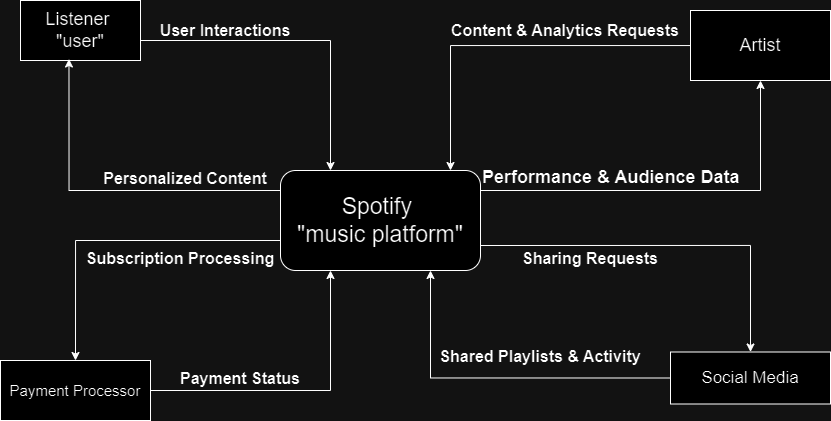
\includegraphics[width=0.8\textwidth]{DFD@Dark.drawio.png}
    \caption{DFD Level 0 - Context Diagram for Spotify-like Application}
    \label{fig:dfd-level0}
\end{figure}

\end{document}
